\subsection{Diseño arquitectural}\label{sec:architecture}

El software desarrollado consiste en un \emph{plugin} que extiende la funcionalidad de Paramics, agregándole la capacidad de comportarse como un servidor TraCI, y que permite a Paramics integrarse de manera transparente con el \emph{framewok} VEINS \autocite{sommer_german_dressler}. Este \emph{framework} modificado, en el cual se reemplazó a SUMO por Paramics, se denominó \textbf{PVEINS}, por ``Paramics VEINS''. 

Específicamente, el \emph{plugin} consiste en una implementación parcial de un servidor TraCI, el cual interpreta mensajes entrantes a través de un \emph{socket} TCP, ejecuta las acciones solicitadas, y responde a través del mismo medio (figura \ref{fig:pveins_genarch}).

\begin{figure}[tpb]
    \centering
    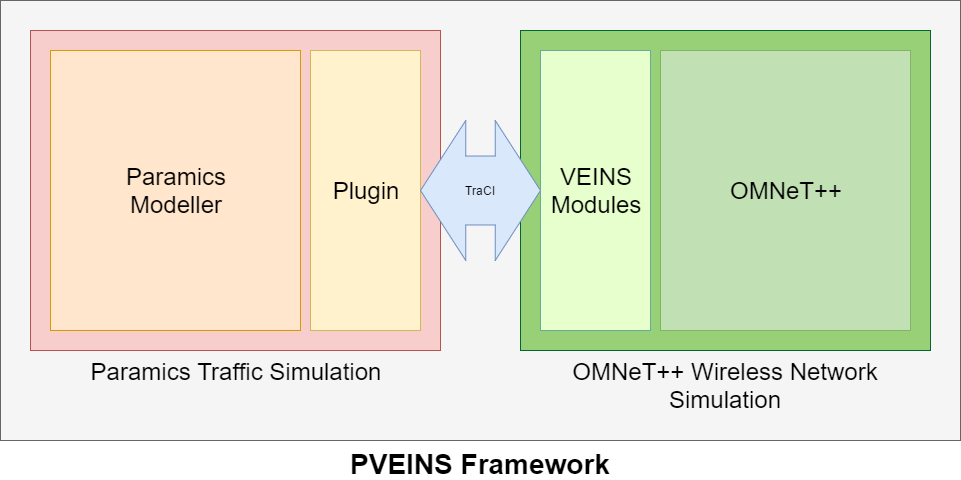
\includegraphics[width=\linewidth]{figuras/PVEINSArch.png}
    \caption[Visión macroscópica del framework]{Visión macroscópica del framework; el plugin desarrollado actúa como una interfaz entre TraCI y Paramics.}
    \label{fig:pveins_genarch}
\end{figure}

A nivel más microscópico, la arquitectura del \emph{framework} se desarrolló en dos versiones distintas, la primera de éstas siendo descartada al realizar las pruebas de validación del proyecto. A continuación, se describirán brevemente estas dos iteraciones del diseño del software, destacando principalmente las razones del descarte de la versión preliminar.

\subsubsection{Arquitectura preliminar}

Originalmente, el \emph{framework} se implementó como un hilo de ejecución (un \emph{thread}) paralelo a Paramics. La principal ventaja de este diseño era evitar el bloqueo de la interfaz del simulador al encontrarse el servidor TraCI bloqueado esperando mensajes entrantes en el \emph{socket}. 

Un diagrama de la arquitectura general de esta implementación puede observarse en la figura \ref{fig:ptraci_arch}. Al iniciar Paramics, el \emph{plugin} inicializa el servidor en un \emph{thread} paralelo; el servidor luego se enlaza a un \emph{socket} TCP y se bloquea en espera de mensajes entrantes desde un cliente TraCI (en nuestro caso, VEINS). Al recibir una serie de comandos TraCI, el servidor los interpreta, comunicándose con Paramics a través de su API, obteniendo datos y modificando el estado de la simulación. El servidor interpreta todos los comandos en un mensaje TraCI antes de enviar todos los mensajes de respuesta correspondientes en un único mensaje TraCI.

Esta arquitectura funciona de manera eficiente y permite la ejecución de la simulación de Paramics completamente sin la intervención del usuario (ya que el \emph{thread} mismo del \emph{plugin} era capaz de llamar el método de inicio de simulación). 

Sin embargo, al comenzar a realizar pruebas con redes de tamaño más extenso se presentó un problema imprevisto, y -- a la larga -- irreparable sin acceso al código fuente de Paramics. El problema radica en la función de avance de simulación definido en la API de Paramics, \texttt{qps\_GUI\_runSimulation()}, la cual, como se descubrió, también actualiza la interfaz gráfica de el modelador de Paramics a través de llamados a la librería Qt4 \cite{qt}. Estos llamados no son \emph{thread-safe}\footnote{Es decir, no incluyen medidas para asegurar el acceso exclusivo de recursos a un sólo \emph{thread}.}, y en redes grandes de Paramics generan \emph{data races} al ser invocados desde un \emph{thread} paralelo al principal del simulador. Esto finalmente genera corrupción de memoria en el motor gráfico (principalmente, lecturas de direcciones inválidas de memoria), lo cual causa un error fatal en la simulación.

Se estudiaron múltiples maneras de resolver este problema manteniendo la estructura paralela del \emph{plugin} sin éxito, ya que la única manera confiable de forzar un avance de la simulación desde el \emph{plugin} es a través de la función anteriormente mencionada. Se decidió entonces abordar el problema desde un ángulo distinto, enfoque que se discutirá en la siguiente sección.

\begin{figure}[]
    \centering
    \begin{sequencediagram}
    \newthread{D}{OMNeT++}{}
    \newinst[1]{A}{VEINS}{}
    \newinst[3]{B}{Plugin (TraCIServer)}{}
    \newthread[2]{C}{Paramics}{}
    
    \begin{messcall}{C}{run()}{B}
        \postlevel
        \begin{call}{B}{waitForCommands()}{B}{}
        \end{call}
    \end{messcall}
    
    \begin{call}{D}{Solicitud}{A}{Resultado}
    
        \begin{call}{A}{Comando TraCI}{B}{Respuesta TraCI}
            \begin{call}{B}{parseCommand()}{B}{sendResponse()}
                \postlevel
                \begin{call}{B}{API Paramics}{C}{Datos}
                \end{call}
                \postlevel
            \end{call}
        \end{call}
    \end{call}
\end{sequencediagram}
    \caption{Arquitectura preliminar.}
    \label{fig:ptraci_arch}
\end{figure}

\subsubsection{Arquitectura final} \label{sec:architecture:final}

El problema presentado por la incompatibilidad de \texttt{qps\_GUI\_runSimulation()}, función de avance de simulación de la API de Paramics, con múltiples \emph{threads} implicó la necesidad de reevaluar la arquitectura general del \emph{framework}. Se decidió descartar la idea de un \emph{thread} paralelo para el servidor, y se implementó un esquema secuencial de interpretación de mensajes TraCI, utilizando \emph{loops} bloqueantes para controlar la ejecución de pasos de simulación.

Esta arquitectura puede visualizarse en la figura \ref{fig:ptraci_arch2}. Al principio de cada paso de simulación, el simulador invoca la función \texttt{qpx\_CLK\_startOfSimLoop()}, definida en el \emph{plugin}, antes de realizar cualquier otra acción. Esta función a su vez invoca el método \texttt{preStep()} del servidor, dentro del cual se ejecuta un \emph{loop} de interpretación de comandos TraCI (y de envío de respuestas a éstos). Este \emph{loop} se interrumpe al recibir un mensaje de paso de simulación, retornando así de \texttt{preStep()} y \texttt{qpx\_CLK\_startOfSimLoop()}, y liberando al simulador para que realice su procedimiento interno de avance de simulación. 

Luego de realizar el avance de simulación, Paramics invoca la función \texttt{qpx\_CLK\_endOfSimLoop()}, también definida en el \emph{plugin}. Esta invoca a su vez el método \texttt{postStep()} del servidor, el cual se encarga de realizar la recolección de datos post-paso de simulación, de terminar de interpretar eventuales comandos recibidos previo al paso de simulación y de enviar respuestas pendientes al cliente. Finalmente, esta función retorna el control de la ejecución a Paramics, y el ciclo comienza nuevamente.

Mediante esta arquitectura se logró eliminar por completo el problema presentado por \texttt{qps\_GUI\_runSimulation()}, y ya que todo corre en un sólo \emph{thread}, se evita el uso de elementos de sincronización, los cuales pueden agregar \emph{overhead} al procedimiento.

Este nuevo diseño presenta una única desventaja: es necesario el inicio de la simulación de manera manual por parte del usuario, luego de lo cual funciona de manera autónoma. Esto ya que no existe manera de iniciar el \emph{loop} de simulación de Paramics a través de la API sin recurrir a \emph{threads}.

Finalmente, se debe notar que dada la representación en tiempo discreto de los pasos de simulación, el avance de esta en muchos casos no alcanza exactamente el tiempo deseado. Si definimos el paso de simulación como $\triangle T$, el instante de tiempo en que se recibe el comando de avance como $T_{i}$ y el instante de tiempo objetivo $T_{o}$, la simulación se avanzará un número $n \in \mathbb{N}$ de pasos, tal que

\begin{multicols}{2}
    \[ T_{i} + (n \times \triangle T) = T_{f} \]
    \[ T_{f} \geq T_{o} \]
    
    \[ T_{i} + ((n - 1) \times \triangle T) = T_{f}' \]
    \[ T_{f}' < T_{o} \]
\end{multicols}

En otras palabras, la simulación se avanzará el mínimo número de pasos tal que el tiempo final es \emph{igual o mayor} al instante de tiempo objetivo. Esto es para asegurar que se ejecuten todas las acciones que dependan del tiempo de simulación por lo menos hasta dicho instante.

\begin{figure}[htpb]
    \centering
    \begin{sequencediagram}
    \newthread{B}{Paramics + Plugin}{}
    \newthread[7]{A}{OMNeT++/VEINS}{}

    \begin{sdblock}{Loop de simulación}{}
        \postlevel
        \begin{call}{B}{\texttt{qpx\_CLK\_startOfSimLoop()}}{B}{}
            \begin{sdblock}{Loop pre-simulación}{}
                \begin{call}{B}{\texttt{server->preStep()}}{B}{Comando: Paso de Simulación}
                    \begin{call}{A}{Mensajes TraCI}{B}{Respuestas TraCI}
                        \postlevel
                    \end{call}
                \end{call}
            \end{sdblock}
        \end{call}
        \begin{sdblock}{Paso de simulación}{}
            \postlevel
            \postlevel
            \begin{call}{B}{\begin{minipage}{8cm}
                        Actualización de estado:
                        \begin{itemize}
                            \item Salida y llegada de vehículos
                            \item Modificación de velocidades y rutas
                        \end{itemize}
                \end{minipage}}{B}{}
            \end{call}
        \end{sdblock}
        \postlevel
        \begin{call}{B}{\texttt{qpx\_CLK\_endOfSimLoop()}}{B}{}
            \begin{sdblock}{Loop post-simulación}{}
                \begin{call}{B}{\texttt{server->postStep()}}{B}{Fin de Comandos}
                    \begin{call}{A}{Mensajes TraCI}{B}{Respuestas TraCI}
                        \postlevel
                    \end{call}
                \end{call}
            \end{sdblock}
        \end{call}
    \end{sdblock}
\end{sequencediagram}
    \caption{Arquitectura final del \emph{framework}}
    \label{fig:ptraci_arch2}
\end{figure}